\documentclass[]{politex}
% ========== Opções ==========
% pnumromarab - Numeração de páginas usando algarismos romanos na parte pré-textual e arábicos na parte textual
% abnttoc - Forçar paginação no sumário conforme ABNT (inclui "p." na frente das páginas)
% normalnum - Numeração contínua de figuras e tabelas 
%	(caso contrário, a numeração é reiniciada a cada capítulo)
% draftprint - Ajusta as margens para impressão de rascunhos
%	(reduz a margem interna)
% twosideprint - Ajusta as margens para impressão frente e verso
% capsec - Forçar letras maiúsculas no título das seções
% espacosimples - Documento usando espaçamento simples
% espacoduplo - Documento usando espaçamento duplo
%	(o padrão é usar espaçamento 1.5)
% times - Tenta usar a fonte Times New Roman para o corpo do texto
% noindentfirst - Não indenta o primeiro parágrafo dos capítulos/seções


% ========== Packages ==========
\usepackage[utf8]{inputenc}
\usepackage{amsmath,amsthm,amsfonts,amssymb}
\usepackage{graphicx,cite,enumerate}


% ========== Language options ==========
\usepackage[brazil]{babel}
%\usepackage[english]{babel}


% ========== ABNT (requer ABNTeX 2) ==========
%	http://www.ctan.org/tex-archive/macros/latex/contrib/abntex2
\usepackage[num]{abntex2cite}

% Forçar o abntex2 a usar [ ] nas referências ao invés de ( )
%\citebrackets{[}{]}


% ========== Lorem ipsum ==========
\usepackage{blindtext}



% ========== Opções do documento ==========
% Título
\titulo{Título}

% Autor
\autor{Lucas Arthur Felgueiras}

% Para múltiplos autores (TCC)
%\autor{Nome Sobrenome\\%
%		Nome Sobrenome\\%
%		Nome Sobrenome}

% Orientador / Coorientador
\orientador{Prof. Dr. Fabio Levy Siqueira}
% \coorientador{Nome do coorientador (opcional)}

% Tipo de documento
\tcc{Engenheiro de Computação}
%\dissertacao{Engenharia Elétrica}
%\teseDOC{Engenharia Elétrica}
%\teseLD
%\memorialLD

% Departamento e área de concentração
\departamento{Engenharia de Computação e Sistemas Digitais}
\areaConcentracao{Engenharia de Software}

% Local
\local{São Paulo}

% Ano
\data{2018}




\begin{document}
% ========== Capa e folhas de rosto ==========
\capa
\falsafolhaderosto
\folhaderosto


% ========== Folha de assinaturas (opcional) ==========
%\begin{folhadeaprovacao}
%	\assinatura{Prof.\ X}
%	\assinatura{Prof.\ Y}
%	\assinatura{Prof.\ Z}
%\end{folhadeaprovacao}


% ========== Ficha catalográfica ==========
% Fazer solicitação no site:
%	http://www.poli.usp.br/en/bibliotecas/servicos/catalogacao-na-publicacao.html


% ========== Dedicatória (opcional) ==========
\dedicatoria{Dedicatória}


% ========== Agradecimentos ==========
\begin{agradecimentos}

Thanks...

\end{agradecimentos}


% ========== Epígrafe (opcional) ==========
\epigrafe{%
	\emph{``Epígrafe''}
	\begin{flushright}
		-{}- Autor
	\end{flushright}
}


% ========== Resumo ==========
\begin{resumo}
Resumo...
%
\\[3\baselineskip]
%
\textbf{Palavras-Chave} -- Palavra, Palavra, Palavra, Palavra, Palavra.
\end{resumo}


% ========== Abstract ==========
\begin{abstract}
Abstract...
%
\\[3\baselineskip]
%
\textbf{Keywords} -- Word, Word, Word, Word, Word.
\end{abstract}


% ========== Listas (opcional) ==========
\listadefiguras
\listadetabelas

% ========== Listas definidas pelo usuário (opcional) ==========
\begin{pretextualsection}{Lista de símbolos}

Lista de símbolos...

\end{pretextualsection}

% ========== Sumário ==========
\sumario



% ========== Elementos textuais ==========

\part{Introdução}

\chapter{Objetivo}
\capepigrafe[0.5\textwidth]{First to mind when asked what 'the cloud' is, a majority respond it’s either an actual cloud, the sky, or something related to weather.}{Citrix Cloud Survey Guide\cite{quotes}}

Com o desenvolvimento da computação, novos programas foram criados, cada vez mais consumindo recursos e sendo hospedados em máquinas pessoais ou dedicadas, porém sem um gerenciamento inteligente de toda a infraestrutura. Além disso, houve a nítida migração de programas \textbf{distribuídos} pela internet para programas que \textbf{rodem} na internet.

\begin{figure}[h!]
  \centering
  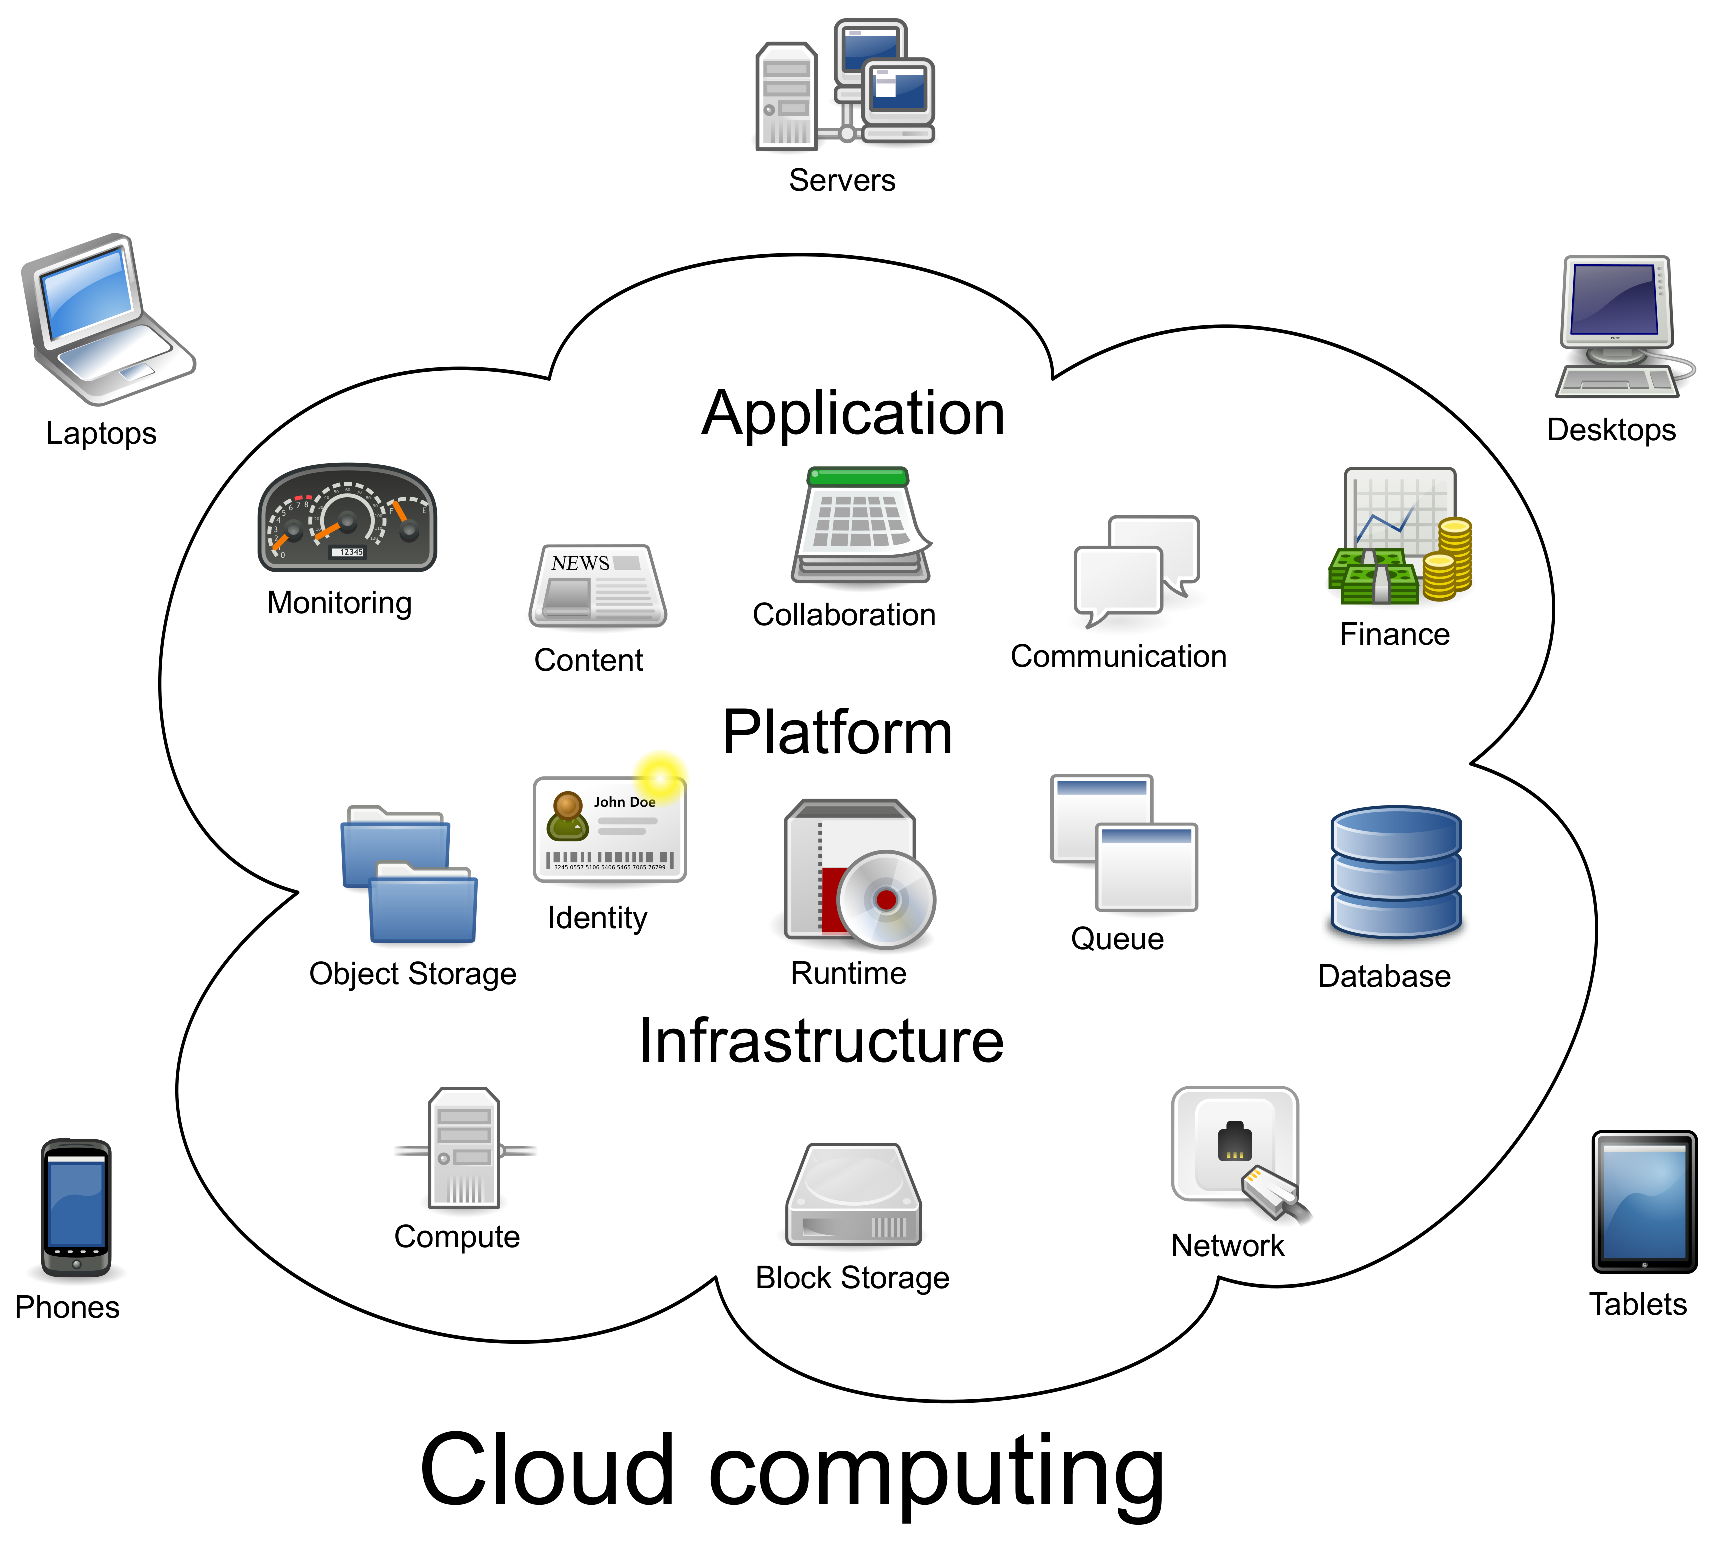
\includegraphics[scale=0.40]{imagens/cloud_computing.eps}
  \caption{Arquitetura Básica de Computação em Nuvem\cite{cloudcomputing}}
\end{figure}

Essas mudanças de paradigma motivaram a criação e consolidação do que conhecemos hoje como Computação em Nuvem, área fortalecida e necessária no desenvolvimento de programas modernos. Ao longo dos pŕoximos capítulos, haverá a explanação em detalhes de como funciona uma arquitetura em nuvem básica, seus desafios técnicos e as principais soluções existentes no mercado.

\chapter{Motivação}

\section{Contexto}
Atualmente, o gerenciamento das duas disciplinas é realizado pelo Tidia-Ae, onde apenas os professores coordenadores da disciplina podem acessar o andamento da matéria, sem a participação dos demais envolvidos, em especial dos orientadores.


\section{Problemas}
Além disso, não há um acompanhamento do status do projeto pelo Tidia-Ae, o que torna ele um simples repositório. O orientador acompanha o andamento do projeto apenas por intermédio do aluno, o que nem sempre gera uma abordagem eficiente, dado que ele depende do retorno do próprio aluno para saber atualizações, além de não ter uma central de fácil acesso para o orientador analisar os documentos relacionados.
  
Por fim, não há um sistema unificado que facilite os alunos que cursam a disciplina de consultar monografias anteriores de maneira estruturada e completamente on-line. O sistema visa, inicialmente, atacar essas demandas, de maneira a melhorar o andamento da disciplina como um todo. Futuramente, pode ser utilizada para outras disciplinas com estruturas semelhantes ao projeto de formatura.

\chapter{Justificativa}

\section{Introdução}
O departamento de Engenharia de Computação e Sistemas Digitais (PCS) da POLI possui duas matérias ao longo do último ano do curso. Cada equipe de alunos (de 1 a 3 pessoas), juntamente com um professor-orientador e um co-orientador (não-obrigatório) elabora um projeto ao longo do ano, para ser avaliado por uma banca teórica e uma feira expositiva, com a recente participação de empresas.

\section{Problemas}
Todo o processo das disciplinas é realizado de maneira manual, com exceção das entregas pontuais. Além disso, os resultados finais são publicados no site da disciplina, após os eventos de avaliação, o que dificulta, por exemplo, a avaliação das empresas. O cálculo final das médias também é manual, gerando trabalho excessivo em pouco tempo aos coordenadores.

\chapter{Organização do Trabalho}
\capepigrafe[0.5\textwidth]{``Frase espirituosa de um autor famoso''}{Autor famoso}

A equipe de desenvolvimento é composta apenas pelo aluno Lucas Arthur Felgueiras, com a orientação do Prof. Dr. Fábio Levy Siqueira, do Laboratório de Tecnologia de Software. O fato da equipe ser limitada, bem como o teor do projeto, afetou a estratégia de trabalho. Por exemplo, certas metodologias ágeis, como o \textit{Scrum}, não poderiam ser utilizadas.

\begin{citacaoLonga}
  \blindtext
\end{citacaoLonga}

\blindtext


\part{Aspectos Conceituais}
\part{Tecnologias Utilizadas}
\part{Metodologia de Trabalho}

% \chapter{Levantamento de Requisitos}
\capepigrafe[0.5\textwidth]{``Frase espirituosa de um autor famoso''}{Autor famoso}

Aqui vem o resumo do capítulo 3 do livro Use Case Modeling

\begin{citacaoLonga}
  \blindtext
\end{citacaoLonga}

\blindtext


\part{Especificação de Requisitos do Sistema}
\part{Projeto e Implementação}
\part{Testes e Implementação}
\part{Considerações Finais}

% \include{conclusoes_projeto_formatura}
% \include{contribuicoes}
% \include{perspectivas_continuidade}
	
\chapter{Capítulo com epígrafe}
\capepigrafe[0.5\textwidth]{``Frase espirituosa de um autor famoso''}{Autor famoso}

\blindtext

\begin{citacaoLonga}
	\blindtext
\end{citacaoLonga}

\blindtext



\blinddocument


% ========== Referências ==========
% --- IEEE ---
%	http://www.ctan.org/tex-archive/macros/latex/contrib/IEEEtran
%\bibliographystyle{IEEEbib}

% --- ABNT (requer ABNTeX 2) ---
%	http://www.ctan.org/tex-archive/macros/latex/contrib/abntex2
%\bibliographystyle{abntex2-num}

%\bibliography{}


% ========== Apêndices (opcional) ==========
\apendice
\chapter{}
\chapter{Beta}


% ========== Anexos (opcional) ==========
\anexo
\chapter{Alpha}
\chapter{}

\end{document}
